
In this chapter, we present the running times of the algorithms. We conducted benchmarks based on well-known instance generators, including Netgen \cite{netgen} and Gridgen \cite{gridgen}.
% as well as datasets from the Bonn benchmark library \cite{bonnmcf}.

The implementations of the algorithms follow the descriptions provided in previous chapters. For Orlin's algorithm, due to the network transformation into an uncapacitated form, we apply a specific heuristic: it iterates over all nodes added during the transformation and pushes $\Delta$ units of flow along the zero-cost edges. This operation significantly improves the running time.

\section{Running times and graphs}

In this section, we present the running times of the algorithms for instances generated by Netgen and Gridgen. Let $n$ denote the number of nodes and $m$ the number of arcs in the network. The test cases are divided into the following groups:

\begin{enumerate}
    \item 8-density ($m = 8n$),
    \item $\sqrt{n}$-density ($m = n\sqrt{n}$),
    \item increasing arc number (increasing $m$ with a constant $n$),
    \item increasing arc capacities (with $m = 8n$), 
    \item increasing arc costs (with $m = 8n$), 
    \item increasing source and target nodes (with $m = 8n$),
    \item a TCT benchmark \cite{bonnmcf}.
\end{enumerate}

All test cases were executed on a machine equipped with an Intel Core i7-6850K processor running at 3.2 GHz.

\subsection{8-density}
This subsection presents the running times for test cases where the number of arcs is fixed at $m = 8n$. \Cref{fig:axis-8} illustrates the results for instances generated by Netgen and Gridgen.

\begin{figure}[H]
    \centering
    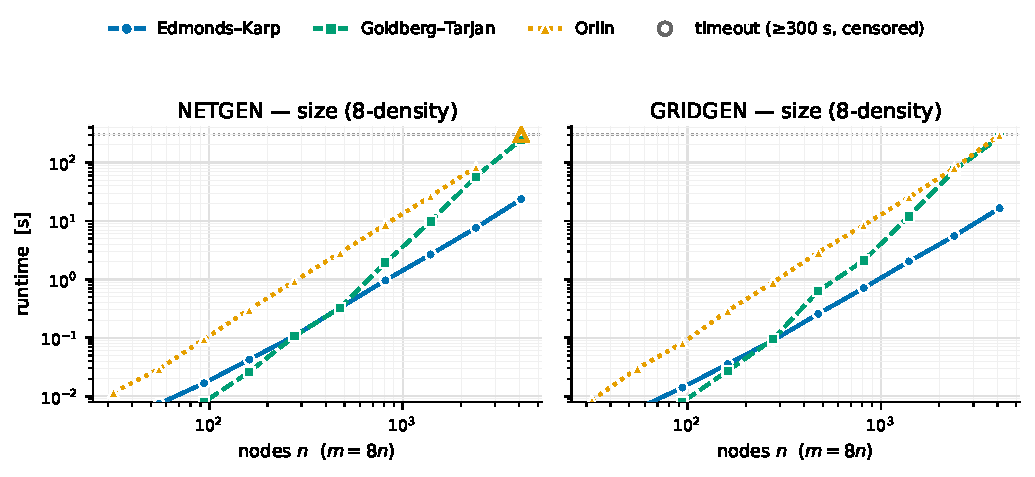
\includegraphics[width=\linewidth]{chapters/benchmarks/figs/axis_size.pdf}
    \caption{Running time graphs for test cases satisfying $m = 8n$.}
    \label{fig:axis-8}
\end{figure}

\subsection{\texorpdfstring{$\sqrt{n}$}{sqrt(n)}-density}
This subsection presents the running times for test cases where the number of arcs satisfies $m = n\sqrt{n}$. The results are illustrated in \Cref{fig:axis-sr}.

\begin{figure}[H]
    \centering
    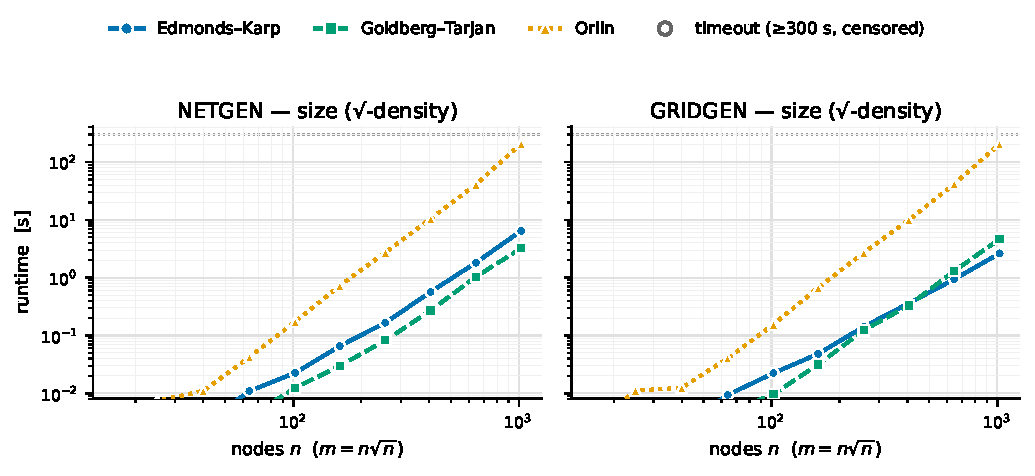
\includegraphics[width=\linewidth]{chapters/benchmarks/figs/axis_sr.pdf}
    \caption{Running time graphs for test cases satisfying $m = n\sqrt{n}$.}
    \label{fig:axis-sr}
\end{figure}

\subsection{Increasing arc number}
In this subsection, we present the running times for test cases where the number of nodes is fixed at $n = 1024$, while the number of arcs increases. Notably, the implementation of Goldberg and Tarjan's algorithm is generally faster for instances with a higher number of arcs. The running times of the remaining algorithms increase as expected. These results are illustrated in \Cref{fig:axis-deg}.

\begin{figure}[H]
    \centering
    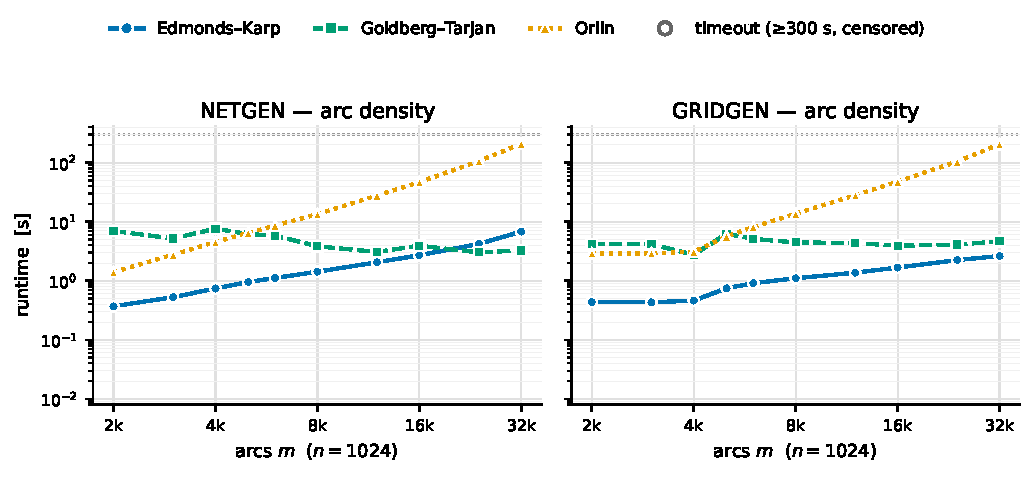
\includegraphics[width=\linewidth]{chapters/benchmarks/figs/axis_deg.pdf}
    \caption{Running time graphs for a constant number of nodes $n$ and an increasing number of arcs $m$.}
    \label{fig:axis-deg}
\end{figure}

\subsection{Increasing capacities}
This subsection details the running times for test cases with increasing arc capacity bounds. It may be surprising that the Edmonds-Karp algorithm performs faster on the final two tests; this occurs because the arc capacities exceed the total supply and demand at the nodes. The running times are illustrated in \Cref{fig:axis-cap}.

\begin{figure}[H]
    \centering
    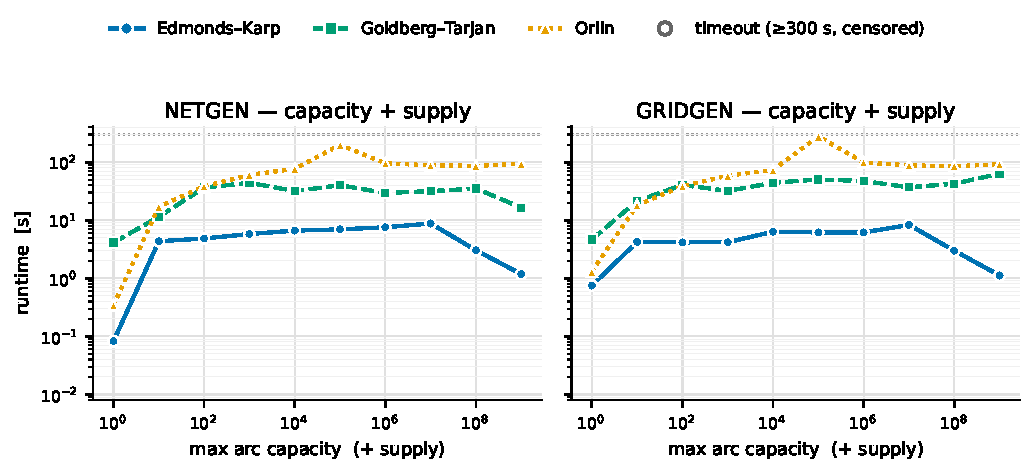
\includegraphics[width=\linewidth]{chapters/benchmarks/figs/axis_cap.pdf}
    \caption{Running time graphs for varying arc capacity bounds and increasing supply/demand among all vertices.}
    \label{fig:axis-cap}
\end{figure}

\subsection{Increasing costs}
Here, we present the running times for test cases with increasing arc cost bounds. The running time of Goldberg and Tarjan's algorithm increases alongside the maximum arc cost. Because the time complexity of this algorithm depends on the cost, this behavior is entirely expected. The other algorithms exhibit relatively unchanged running times across all test instances, as their performance does not strictly depend on arc costs. These results are illustrated in \Cref{fig:axis-cost}.

\begin{figure}[H]
    \centering
    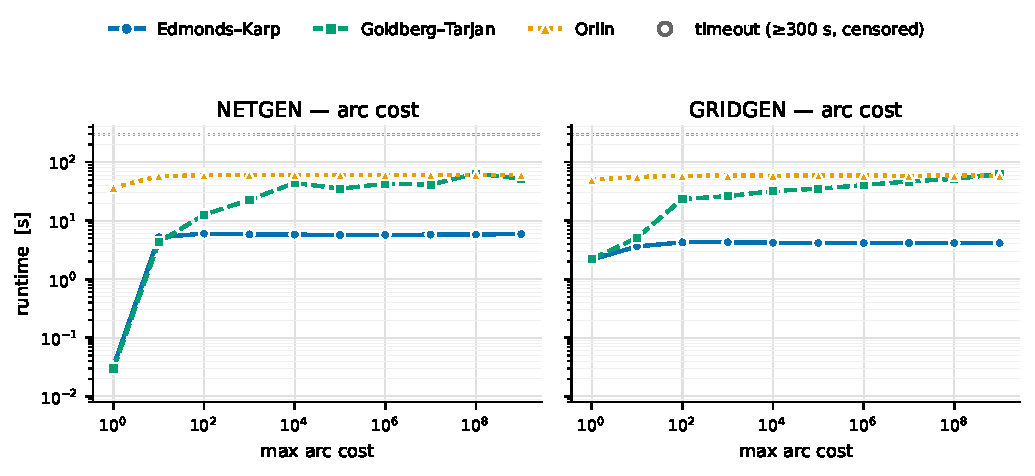
\includegraphics[width=\linewidth]{chapters/benchmarks/figs/axis_cost.pdf}
    \caption{Running time graphs for increasing arc cost bounds.}
    \label{fig:axis-cost}
\end{figure}

\subsection{Increasing source and target nodes}
This subsection presents the running times for test cases where the number of supply and demand nodes increases. The motivation for this benchmark stems from the observation that Orlin's algorithm can be slower due to the increased number of vertices and supply/demand nodes resulting from the uncapacitated network transformation. We aimed to determine whether a large number of supply or demand nodes would cause a significant difference in performance. However, as illustrated in \Cref{fig:axis-sd}, the running times remain relatively stable without major variations.

\begin{figure}[H]
    \centering
    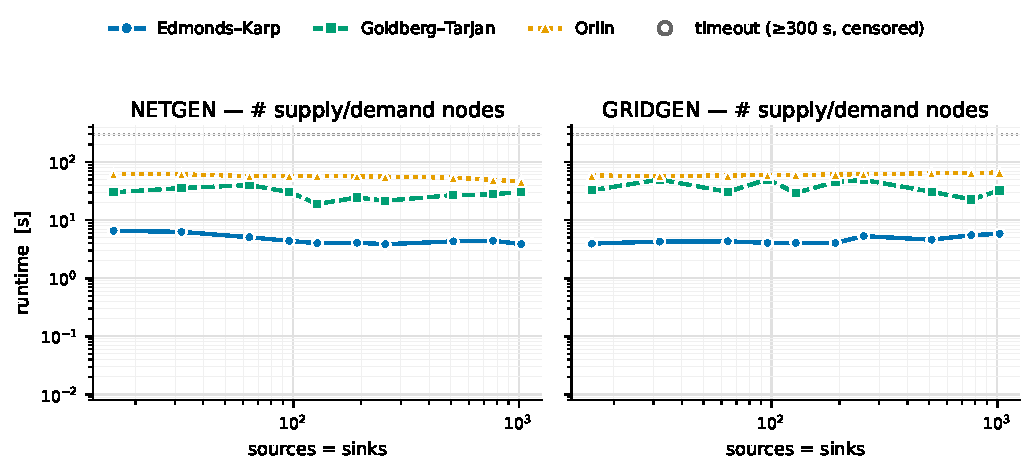
\includegraphics[width=\linewidth]{chapters/benchmarks/figs/axis_sd.pdf}
    \caption{Running time graphs for an increasing number of source and target nodes.}
    \label{fig:axis-sd}
\end{figure}

\subsection{TCT benchmark}

The TCT benchmarks represent a linear relaxation of the time-cost tradeoff problem in \textit{VLSI threshold voltage assignment}. It is a design technique that assigns voltages to transistors, minimizing the static leakage power without violating timing constraints. This problem can be modeled as a minimum cost flow problem.

The following test cases are taken from \textit{Large Benchmarks for the Minimum-Cost Flow Problem} \cite{bonnmcf}.

\begin{table}[htbp]
    \centering
    \caption{TCT Benchmark Instances: Graph Properties}
    \label{tab:tct_graph_sizes}
    \begin{tabular}{lrr}
        \toprule
        \textbf{Testcase File} & \textbf{Nodes ($V$)} & \textbf{Arcs ($E$)} \\
        \midrule
        TCTS.dimacs & 5,947 & 14,907 \\
        TCTL.dimacs & 623,632 & 1,234,893 \\
        TCTB.dimacs & 936,216 & 2,114,029 \\
        TCTD.dimacs & 1,650,760 & 3,491,477 \\
        TCTM.dimacs & 3,393,802 & 7,528,057 \\
        TCTV.dimacs & 11,506,694 & 24,544,169 \\
        \bottomrule
    \end{tabular}
\end{table}

The results are shown in \Cref{tab:tct_benchmarks_cpu_projected}. Goldberg and Tarjan's algorithm is far better for these instances than the other tested algorithms. The reason for the significant time difference is the different algorithmic approach. The capacity scaling algorithm is highly inefficient in this case.

\begin{table}[htbp]
    \centering
    \caption{TCT MCF Benchmark Results: CPU Time (Limit: 3h)}
    \label{tab:tct_benchmarks_cpu_projected}
    \begin{tabular}{lrrr}
        \toprule
        \textbf{Testcase} & \textbf{Edmonds-Karp (s)} & \textbf{Orlin (s)} & \textbf{Goldberg-Tarjan (s)} \\
        \midrule
        TCTS.dimacs & 3.450 & 6.268 & 0.018 \\
        TCTL.dimacs & TLE   & TLE   & 17.452 \\
        TCTB.dimacs & TLE   & TLE   & 36.138 \\
        TCTD.dimacs & TLE   & TLE   & 123.680 \\
        TCTM.dimacs & TLE   & TLE   & 618.628 \\
        TCTV.dimacs & TLE   & TLE   & $\sim$6930.000\rlap{\textsuperscript{$\dagger$}} \\
        \bottomrule
        \multicolumn{4}{l}{\small TLE = Time Limit Exceeded ($>3$h).} \\
        % \multicolumn{4}{l}{\small \textsuperscript{*}Completed during extended time limit testing.} \\
        \multicolumn{4}{l}{\small \textsuperscript{$\dagger$}Projected value based on empirical quadratic scaling ($O((m+n)^2)$).}
    \end{tabular}
\end{table}


\section{Summary}
The Edmonds-Karp capacity scaling algorithm yields the best running times in almost every tested benchmark, though the cost scaling algorithm performs comparably well in many cases.

Although Orlin's algorithm is theoretically faster, its practical implementation is generally much slower compared to other algorithms. The required network transformation appears to be its primary performance bottleneck.

Typically, the most time-consuming operation in Orlin's algorithm is finding augmenting paths. Despite optimizations to the augmenting arcs incident to uncapacitated vertices, the transformed networks remain too large to achieve reasonable running times.

However, if we introduced some uncapacitated instances, Orlin's algorithm would likely be faster compared to the standard capacity scaling algorithm by Edmonds and Karp, as the network transformation would not be necessary.

Capacity scaling algorithms may also be more efficient for dense networks with a single strongly connected component. The need to augment flow through an artificial node, created to ensure network connectivity, forces us to augment an equal amount of flow outward. Therefore, if a network contains multiple components, the nodes for augmentation must be chosen more carefully.